\documentclass[12pt, letterpaper]{article}
\usepackage{float}
\usepackage{amsmath}
\usepackage{hyperref}
\usepackage{indentfirst}

\usepackage{enumitem}[labelindent=5cm]

\usepackage[bottom]{footmisc}

\usepackage{tikz}
\usepackage{caption}
\usetikzlibrary{matrix, positioning}
\tikzset{bullet/.style={circle,fill,inner sep=2pt}}

\usepackage{graphicx}
\graphicspath{ {./images/} }

\usepackage{geometry}
\geometry{margin=1in}

\begin{document}
\setlength\parindent{1cm}

\title{Binomial Options Pricing Model (CRR Version)\\
\large MATH 3332 - Probability and Inference}
\author{Charlie Liu}
\date{\today}
\maketitle

\section*{Introduction}

In finance and economics, the asset market is a blanket term that covers all the various underlying markets that involve the exchange of financial assets.
The stock market is one popular example of an underlying market where buyers and sellers can exchange assets in the form of stocks/shares (ownership) of a company.
Other notable markets include the bond market where fixed-income assets like corporate bonds are exchanged, and the derivatives market where contracts between two consenting parties are exchanged.
The different types of markets can be accessed depends on the features provided by the service or brokerage used.

\medskip

Since assets exchanged on the market are based on a seller's chosen price, one must account for the valuation of the asset to avoid over paying.
The valuation of an asset is based on the future expected cash flow\cite{damodaran} and is especially important when exchanging assets because pricing is typically determined by the seller and influenced by the buyers.
It is important to note here that because asset valuation is based on future expected cash flow, any calculated valuation such as intrinsic/justified valuation is considered theoretical.
This is why quantitative analysis is heavily used in asset valuation as the various mathematical models and technicals/fundamentals are used to estimate the valution of an asset.
For stocks and bonds, there are various ways to obtain the intrinsic value through different mathematical models.
These will not be covered in this paper, but some of them can be viewed on Obaidullah's stock valuations article\cite{obaidullahxplaind}.

\medskip

For financial derivatives, valuation is a lot harder to calculate because they are essentially contracts that \textit{derive} their value from the performance of the underlying entity\cite{derivativefinancewikipedia}, thus various factors in addition to the factors affecting the underlying stock value can alter the valuation of the option contract. 

\medskip

In this paper, we will focus on a specific financial derivative called the options contract with stocks as its derivation.
An options contract gives the buyer the right to ``exercise" the contract which means the contract holder can either buy or sell the ${x}$ number\footnote{The number of underlying stock in a single option is usually 100 stocks.} of underlying stock at a fixed price called the stike price once the underlying stock's price passes the strike price\footnote{In the case of "puts" (right to sell), the stock's price must be lower than the strike price. In the case of "calls" (right to buy), the stock's price must be higher than the strike price. }.
They are essentially reservations to buy or sell ${x}$ number of stock.
In order to profit from exercising the option, the amount generated from buying or selling at the strike price must cover the cost of the option.
All option contracts come with an expiration time\footnote{Also known as ``maturity"}.
If the strike price condition is not met for the option contract, then the contract will ``expire" and is considered worthless because the owner of the option can get a better deal at market price instead of the option's strike price.
An option contract to buy the underlying entity is called a call and an option contract to sell the underlying entity is called a put.
One may buy a call or put option on the market and then sell that same option contract on the market.

\medskip

The famous mathematical model called the Black-Scholes Model developed by Fischer Black, Myron Scholes, and Robert C. Merton was able to give a theoretical valuation of European-style options \cite{blackscholesmodelwikipedia}.
There is emphasis on ``European-style" options in this case because the Black-Scholes model (by itself) is only accurate on the European-style options.
European-style options only allow exercise on expiration, while American-style options allow the holder to exercise before expiration.
This early exercise of the American-style options makes it difficult to find the optimal time to exercise the option for maximum gains \cite{blackscholesmodelwikipedia} as the Black-Scholes model cannot account for the various outcomes before expiration. 

\medskip

The binomial options pricing model overcame this limitation for the American-style options \cite{bopmwikipedia}.
Its main feature of generating ``nodes" that represent different possible outcomes over a period of time allows for better insight into the optimal stop.
It was originally proposed by William Sharpe in 1978, but was formalized in 1979 by John Carrington Cox, Stephen Ross, and Mark Edward Rubenstein \cite{bopmwikipedia}.

\medskip

The name ``binomial options pricing model" is a generic name that encompasses all forms\footnote{different versions i.e using different formulas} of different binomial options pricing models.
Cox, Ross, and Rubenstein's version of the binomial options pricing model became commonly known as the ``CRR model" \cite{thebinomialmodelcornell}.

\medskip

In this paper, ``binomial options pricing model" will be synonymous to the CRR model and for the sake of keeping consistency and simplicity, all formulas and calculations demonstrated here will be based on the CRR model.

\pagebreak

\section*{Methods}

The binomial options pricing model aims to find the valuation of the chosen option at discrete times based on various inputs given.
It achieves this by generating a binomial decision tree\footnote{Technically a lattice.} where each node represents the valuation of the option at a certain point in time.
This binomial lattice is composed of Bernoulli processes because at each (non end/start) node there are two directional outcomes of the stock: up or down.
This also means that the probabilities for up and down movement are ${p}$ and ${1-p}$ respectively where ${0 \leq p \leq 1}$. 
Figure \ref{fig:genericlattice} gives a generalized 2-period example of a binomial options lattice this:
\begin{figure}[H]
  \centering
  \begin{tikzpicture}[>=stealth, sloped, baseline]
    \matrix (tree) [%
      matrix of nodes,
      minimum size=1cm,
      column sep=2cm,
      row sep=1.2cm, nodes={text width=5em}
      	]
      {
  		  t=0 & t=1 & t=2 \\
  
            &  &  {} \\
  
        	&  {}  &\\
  
        {}  &  &  {}\\
  
        	&  {}  &\\
  
            &  &  {} \\
      };
      \node[bullet, left=0mm of tree-2-3.west,
        label={[label distance=1mm]90:${u^2S}$},
        label={[label distance=2mm]0:${EV_{2,n}}$},
        label={[label distance=2mm]270:${BV_{2,n}}$}
        ](b-2-3){};

      \node[bullet, left=0mm of tree-3-2.west,
        label={[label distance=1mm]90:${uS}$},
        label={[label distance=2mm]0:${EV_{1,n}}$},
        label={[label distance=2mm]270:${BV_{1,n}}$}
        ](b-3-2){};

      \node[bullet, right=7mm of tree-4-1.west,
        label={[label distance=1mm]90:${S_0}$},
        label={[label distance=2mm]0:${EV_{0,n}}$},
        label={[label distance=2mm]270:${BV_{0,n}}$}
        ](b-4-1){};

      \node[bullet, left=0mm of tree-4-3.west,
        label={[label distance=1mm]90:${udS}$},
        label={[label distance=2mm]0:${EV_{2,n}}$},
        label={[label distance=2mm]270:${BV_{2,n}}$}
        ](b-4-3){};

      \node[bullet, left=0mm of tree-5-2.west,
        label={[label distance=1mm]90:${dS}$},
        label={[label distance=2mm]0:${EV_{1,n}}$},
        label={[label distance=2mm]270:${BV_{1,n}}$}
        ](b-5-2){};

      \node[bullet, left=0mm of tree-6-3.west,
        label={[label distance=1mm]90:${u^2S}$},
        label={[label distance=2mm]0:${EV_{2,n}}$},
        label={[label distance=2mm]270:${BV_{2,n}}$}
        ](b-6-3){};

      \draw[->] (b-4-1) -- (b-3-2) node [midway,above] {$p$};
      \draw[->] (b-4-1) -- (b-5-2) node [midway,below] {$(1-p)$};
      
  		\draw[->] (b-3-2) -- (b-2-3) node [midway,above] {$p$};
      \draw[->] (b-3-2) -- (b-4-3) node [midway,below] {$(1-p)$};
  
  		\draw[->] (b-5-2) -- (b-4-3) node [midway,above] {$p$};
      \draw[->] (b-5-2) -- (b-6-3) node [midway,below] {$(1-p)$};
  \end{tikzpicture}
  \caption{A generic binomial options pricing lattice with 2 periods}
  \label{fig:genericlattice}
\end{figure}

\pagebreak
There are multiple ways to obtain the valuation of the option using this model.
The novel feature of this model is that option valuation can be achieved without the need of probabilities.
This same feature is what made Black-Scholes famous in that the true probabilities and expected returns were uneccessary to obtain the valuation of the given option contract\cite{brigidavideo}.
Two arbitrage-free pricing methods through ``delta-hedging" and replicating portfolio can achieve the same valuation and both of which do not need the probabilities at each outcome.
Both of these methods are outside the scope of this paper, and the instead this paper will focus on the probability method used to obtain the value of an option.

\bigskip

The process to evaluate the given option is described as a three step process\cite{bopmwikipedia}:
\begin{enumerate}[leftmargin=2\parindent]
  \item Price tree generation
  \item Calculation of option value at each final node
  \item Sequential calculation of the option value at each preceding node
\end{enumerate}

\bigskip

To best describe this method, it's best to have an example.
Here are some variables that need to be established:

\begin{itemize}[label={}]
  \item Let \textit{\textbf{Stock Price(S)}} = 100
  \item Let \textit{\textbf{Strike Price(X)}} = 120
  \item Let \textit{\textbf{Risk-Free Interest Rate(r)}} = 0.09\%
  \item Let \textit{\textbf{Up Factor(u)}} = 1.25
  \item Let \textit{\textbf{Down Factor(d)}} = ${\frac{1}{u} = \frac{1}{1.25} = 0.80}$
  \item Let \textit{\textbf{Time in Year(s) (T)}}  = 1
  \item Let \textit{\textbf{Time Periods (t)}}  = 2 
\end{itemize}

\bigskip

Explaination for the newly introduced variables:
\begin{itemize}[label={}]
  \item \textbf{Risk-Free Interest Rate} - Will be explained in the upcoming section
  \item \textbf{Up Factor} - The factor that the stock price moves up at for each period (t)
  \item \textbf{Down Factor} - The factor that the stock price moves down at for each period (t)
  \item \textbf{Time in Years} - The duration of the entire model in years\footnote{So if our duration is 0.5, then our entire model is lasting half a year}.
  \item \textbf{Time Periods} - The number of time periods (generations) in a generated binomial options pricing model
\end{itemize}

\pagebreak
\subsection*{1. Price Tree Generation}
\subsubsection*{Establishing Movement Factors}
The initial step in generating the lattice is to obtain the up(${u}$) and down(${d}$) factors. From the original 1979 CRR paper, the up and down factors are calculated using\cite{bopmwikipedia}\cite{crrpaper}:
\begin{align*}
    u &= e^{\sigma\sqrt{t/n}} \\
    d &= e^{-\sigma\sqrt{t/n}} = \frac{1}{u} \\
    \text{where}~\sigma &= \text{the volatility (standard deviation) of the stock price} \\
    t &= \text{the duration\footnote{This is essentially the value of $\frac{T}/{t}$ where ${t}$ in this case is the number of periods in the model}of time period} \\
    n &= \text{the duration\footnote{The both durations must have the same unit of time} until expiration}
\end{align*}

\medskip

The rate of increase in the factors: ${\sigma\sqrt{2/\pi}}$ and ${-\sigma\sqrt{t/n}}$ were \textit{probably} derived from the mean absolute deviation (MAD) formula since both fomulas bear a resemblence to the MAD's formula\cite{madwikipedia}:
\begin{equation*}
  MAD = \sigma\sqrt{2/\pi}
\end{equation*}

\noindent Which seems reasonable to believe in this context as both ${u}$ and ${d}$ are essentially compounding the volatility (standard deviation) over a period of time from the initial price of a stock.

\bigskip

One neat thing about these formulas is that the stock price at a certain time period ${n}$ can be calculated with:
\begin{equation*}
  {S}_n = {S}_0 \cdot {u}^{N_u-N_d}
\end{equation*}

Since nodes with paths ${u > d}$:
\begin{equation*}
  \setlength{\jot}{10pt}
  \begin{split}
    {S}_n
    & = {S}_0 \cdot {u}^{N_u-N_d} \\
    & = {S}_0 \cdot {u}^n
  \end{split}
\end{equation*}

Nodes with paths ${u < d}$:
\begin{equation*}
  \setlength{\jot}{10pt}
  \begin{split}
    {S}_n
    & = {S}_0 \cdot {u}^{N_u-N_d} \\
    & = {S}_0 \cdot {u^{-n}} \\
    & = {S}_0 \cdot {1/u^n} \\
    & = {S}_0 \cdot ({1/u})^n \\
    & = {S}_0 \cdot {d^n}
  \end{split}
\end{equation*}

And nodes with paths ${u = d}$:
\begin{equation*}
  \setlength{\jot}{10pt}
  \begin{split}
    {S}_n
    & = {S}_0 \cdot {u}^{N_u-N_d} \\
    & = {S}_0 \cdot {u^0} \\
    & = {S}_0 \cdot 1 \\
    & = {S}_0
  \end{split}
\end{equation*}

These formulas are derived from the continous compouding formula\cite{continouscompoundingformulawikipedia}\cite{exponentcharacterizationswikipedia}:
${P(t)} = {P}_{0}e^{rt}$
because the value at each consecutive node is essentially the initial value of the stock compounded by the value of the stock influenced by the movement factor at a certain period.


\subsubsection*{Risk-free interest rate}
Risk-free\footnote{Realistically, there's probably nothing that's truly risk-free unless it's arbitrage} interest rate is the value that represents the safest interest yield one would earn if they were to put the money in that asset.
The most common risk-free interest used is the U.S Treasury bond yields as the bonds are considered the safest\footnote{The risk is so low that its negligible} assets to obtain interest.

For simplicity, this paper will use 0.09\%\footnote{This was the yield listed on November 25, 2020} from the current 6-month\footnote{6-months because we have our expiration at 1 year and only 2 time periods i.e 2 6-month periods} U.S Treasury bill as the risk-free interest rate for calculations.

\pagebreak
\subsubsection*{Generated Tree}
Given the variables for this example, the tree with stock price estimates is generated below:
\begin{figure}[H]
  \centering
  \begin{tikzpicture}[>=stealth, sloped, baseline]
    \matrix (tree) [%
      matrix of nodes,
      minimum size=1cm,
      column sep=2cm,
      row sep=1.2cm, nodes={text width=5em}
      	]
      {
  		  t=0 & t=1 & t=2 \\
  
  					&  &  {} \\
  
        	&  {}  &\\
  
        {}  &  &  {}\\
  
        	&  {}  &\\
  
  					&  &  {} \\
      };

      \node[bullet, left=0mm of tree-2-3.west,
        label={[label distance=1mm]90:${\$156.25}$},
        label={[label distance=2mm]0:${EV_{2,n}}$},
        label={[label distance=2mm]270:${BV_{2,n}}$}
        ](b-2-3){};

      \node[bullet, left=0mm of tree-3-2.west,
        label={[label distance=1mm]90:${\$125}$},
        label={[label distance=2mm]0:${EV_{1,n}}$},
        label={[label distance=2mm]270:${BV_{1,n}}$}
        ](b-3-2){};

      \node[bullet, right=7mm of tree-4-1.west,
        label={[label distance=1mm]90:${\$100}$},
        label={[label distance=2mm]0:${EV_{0,n}}$},
        label={[label distance=2mm]270:${BV_{0,n}}$}
        ](b-4-1){};

      \node[bullet, left=0mm of tree-4-3.west,
        label={[label distance=1mm]90:${\$100}$},
        label={[label distance=2mm]0:${EV_{2,n}}$},
        label={[label distance=2mm]270:${BV_{2,n}}$}
        ](b-4-3){};

      \node[bullet, left=0mm of tree-5-2.west,
        label={[label distance=1mm]90:${\$80}$},
        label={[label distance=2mm]0:${EV_{1,n}}$},
        label={[label distance=2mm]270:${BV_{1,n}}$}
        ](b-5-2){};

      \node[bullet, left=0mm of tree-6-3.west,
        label={[label distance=1mm]90:${\$64}$},
        label={[label distance=2mm]0:${EV_{2,n}}$},
        label={[label distance=2mm]270:${BV_{2,n}}$}
        ](b-6-3){};

      \draw[->] (b-4-1) -- (b-3-2) node [midway,above] {$p$};
      \draw[->] (b-4-1) -- (b-5-2) node [midway,below] {$(1-p)$};
      
  		\draw[->] (b-3-2) -- (b-2-3) node [midway,above] {$p$};
      \draw[->] (b-3-2) -- (b-4-3) node [midway,below] {$(1-p)$};
  
  		\draw[->] (b-5-2) -- (b-4-3) node [midway,above] {$p$};
      \draw[->] (b-5-2) -- (b-6-3) node [midway,below] {$(1-p)$};
  \end{tikzpicture}
  \caption{The generated binomial tree with stock prices for 2 periods}
\end{figure}


\subsection*{2. Option Exercise Values}
With the price tree generated in Figure 2, the option's exercise\footnote{This is also referred to as the intrinsic (face-value) value} value for each node needs to be found because American-style call options can be exercised at any time before expiration.
For a European-style call option, only the final nodes of the lattice will have the option value because European-style options can only be exercised at expiration. 
The exercise value is calculated \cite{bopmwikipedia} by:
\begin{eqnarray*}
  \text{\textit{Call Option (${EV_t,n}$)}} = Max({S_n - X}, 0) \\
  \text{\textit{Put Option (${EV_t,n}$)}} = Max(0, {X - S_n}) 
\end{eqnarray*}

For a call option, if the difference between the stock price and the strike price (${S_n - X}$) is less than (or equal to) 0, then the option is essentially worthless i.e \$0 because the strike price is the price in which the owner of the call option can purchase the underlying stocks at.
Since the price of the stock on the market is lower than the strike price, it makes no sense for the owner of the call option to exercise the option and buy at the strike price when he or she purchase the shares at a lower price straight from the market.

\medskip

The same is applied for the put option, except put options gives the user the right to sell the underlying stock at the certain strike price, thus the setup for the difference is reversed.
If the difference between the strike price and the stock price (${X - S_n}$) is positive, then it makes sense for the owner to exercise the put option and sell the stocks at the strike price rather than the lower market price.

\bigskip

Our updated tree with the option values are listed below:
\begin{figure}[H]
  \centering
  \begin{tikzpicture}[>=stealth, sloped, baseline]
    \matrix (tree) [%
      matrix of nodes,
      minimum size=1cm,
      column sep=2cm,
      row sep=1.2cm, nodes={text width=5em}
      	]
      {
  		  t=0 & t=1 & t=2 \\
  
  					&  &  {} \\
  
        	&  {}  &\\
  
        {}  &  &  {}\\
  
        	&  {}  &\\
  
  					&  &  {} \\
      };

      \node[bullet, left=0mm of tree-2-3.west,
        label={[label distance=1mm]90:${\$156.25}$},
        label={[label distance=2mm]0:${\$36.25}$},
        label={[label distance=2mm]270:${BV_{2,n}}$}
        ](b-2-3){};

      \node[bullet, left=0mm of tree-3-2.west,
        label={[label distance=1mm]90:${\$125}$},
        label={[label distance=2mm]0:${\$5}$},
        label={[label distance=2mm]270:${BV_{1,n}}$}
        ](b-3-2){};

      \node[bullet, right=7mm of tree-4-1.west,
        label={[label distance=1mm]90:${\$100}$},
        label={[label distance=2mm]0:${\$0}$},
        label={[label distance=2mm]270:${BV_{0,n}}$}
        ](b-4-1){};

      \node[bullet, left=0mm of tree-4-3.west,
        label={[label distance=1mm]90:${\$100}$},
        label={[label distance=2mm]0:${\$0}$},
        label={[label distance=2mm]270:${BV_{2,n}}$}
        ](b-4-3){};

      \node[bullet, left=0mm of tree-5-2.west,
        label={[label distance=1mm]90:${\$80}$},
        label={[label distance=2mm]0:${\$0}$},
        label={[label distance=2mm]270:${BV_{1,n}}$}
        ](b-5-2){};

      \node[bullet, left=0mm of tree-6-3.west,
        label={[label distance=1mm]90:${\$64}$},
        label={[label distance=2mm]0:${\$0}$},
        label={[label distance=2mm]270:${BV_{2,n}}$}
        ](b-6-3){};

      \draw[->] (b-4-1) -- (b-3-2) node [midway,above] {$p$};
      \draw[->] (b-4-1) -- (b-5-2) node [midway,below] {$(1-p)$};
      
  		\draw[->] (b-3-2) -- (b-2-3) node [midway,above] {$p$};
      \draw[->] (b-3-2) -- (b-4-3) node [midway,below] {$(1-p)$};
  
  		\draw[->] (b-5-2) -- (b-4-3) node [midway,above] {$p$};
      \draw[->] (b-5-2) -- (b-6-3) node [midway,below] {$(1-p)$};
  \end{tikzpicture}
  \caption{Updated tree with option value at the end of the 2 periods}
\end{figure}

\pagebreak
\subsection*{3. Backward Induction for Binomial Values}
With the exercise values calculated in the previous step, backward induction is used to obtain the option values at each node starting from the nodes before expiration/last.
This value calculated is called the "binomial value" and is calculated from the "risk neutral valuation".

\subsubsection*{Risk neutral valuation}
%(https://en.wikipedia.org/wiki/Rational_pricing#Risk_neutral_valuation)
The risk neutral valuation is the valution of an option with risk neutrality assumption.

Risk neutrality assumption is based on the risk-neutral measure which is in-turn based on the fundamental theorem of asset pricing which implies that today's value is the discounted expected value of a future payoff.
%(https://youtu.be/eG_aRPy1KVE?t=1353) (https://en.wikipedia.org/wiki/Risk-neutral_measure)

The idea of the risk-neutral measure is that it is a probability measure that takes into consideration all future outcomes including the risks involved under its probability distribtion.


\subsubsection*{Arbitrage}
Arbitrage in the simplest terms is taking profit with no risk (a common form of it is profiting from price difference on different markets).
For the math behind risk-neutral valuation to work, we must assume that there is no arbitrage.

We need to confirm these statements to be true:
\begin{align*}
  & {r > 0} \\
  & S_d \leq (1+r)S \leq S_u
\end{align*}


\subsubsection*{Binomial Value}
The binomial value is calculated by:
\begin{align*}
  & V_{t-\Delta t, n} = \frac{[(p)V_{t,n} + (1-p)V_{t,n+1}]}{e^{r\Delta t}}
  \\
  & \textrm{where "n" is the nodes of a generation (NOT the generation itself!)}
\end{align*}


Which in plain english is:
\begin{equation*}
  \textrm{\textit{Present Option Value (PV)}} = \frac{\textrm{[${p}$ ${\cdot}$ \textit{Option Up} + (1 - ${p}$) \textit{Option Down}]}}{\textrm{\textit{Compounded risk free interest rate}}}
\end{equation*}

The origin of this formula came from the formula for present value: %[This took me a long time to break down and find out]
\begin{equation*}
  P = \frac{F}{(1+r)^t}
\end{equation*}

Where F represents the future value and in this context will be the expected value of returns from our options at period n:
\begin{equation*}
  F = (p)V_{t,n} + (1-p)V_{t,n+1}
\end{equation*}
and since we know that expected value is countable/discrete because we are calculating based on countable and finite periods, our formula is:
\begin{equation*}
  \setlength{\jot}{10pt}
  \begin{split}
    E[V] 
    & = \sum\limits_{n \in \{u,d\}} p_n V_{t,n} \\
    & = p_1 V_{t,u} + p_2 V_{t,d} \\
    & = (p) V_{t,u} + (1-p) V_{t,d} \\
  \end{split}
\end{equation*}
%(https://www.scranton.edu/faculty/hussain/teaching/fin586_/GPT103.pdf)

\subsubsection*{Probability}
Now that we're given the formula for the binomial value and broken down they reason for the formula, one last unknown to calculate is the probability "p".

This probability is calculated with the formula:
\begin{equation*}
  p = \frac{e^{rt} - d}{u - d}
\end{equation*}

Which is essentially the formula for Andrew D. Roy's ratio to measure market price of risk:
%(https://en.wikipedia.org/wiki/Risk-neutral_measure)
%(https://en.wikipedia.org/wiki/Sharpe_ratio)
%(https://en.wikipedia.org/wiki/Roy%27s_safety-first_criterion)
\begin{equation*}
  \frac{\mu - m}{\sigma}
\end{equation*}

Where $\mu$ is the gross expected return, "m" is the minimum acceptable return (risk), and $\sigma$ is the standard deviation of returns.

By solving for "p" with our given example variables:
\begin{equation*}
  \setlength{\jot}{10pt}
  \begin{split}
    p
    & = \frac{e^{rt} - d}{u - d}
    \\
    & = \frac{(1+r) - d}{u - d}
    \\
    & = \frac{1.0009 - 0.80}{1.25 - 0.80}
    \\
    & = \frac{1.0009 - 0.80}{0.45}
    \\
    & = \frac{0.2009}{0.45}
    \\
    & = 0.6\overline{4}
  \end{split}
\end{equation*}

We can see that the final result fits the formula for market price of risk:
\begin{equation*}
  \frac{\mu - m}{\sigma} = \frac{1.0009 - 0.80}{0.45}
\end{equation*}

Where ${1.0009}$ is the gross minimum expected return from investment based on the risk free interest rate.
If the expected return was lower than the risk-free interest rate, then it makes no sense to invest in an asset with the expectation that the return will be lower than the safest expected return such as treasury bonds.

The minimum acceptable return (m) is ${0.80}$ and is based off of the down factor because that is in the worst case, the amount of return one would get from the underlying purchase.

${\sigma}$, the standard deviation, is ${0.45}$ and that is basically the size of the spread between the up and down outcomes.

Putting these together, the result is something that calculates the probability of getting a minimum acceptable return. %(https://www.investopedia.com/terms/r/roys-safety-first-criterion.asp)

This probability effectively becomes the probability of the option moving up and thus conversely by complement ${(1-p)}$ becomes the probability of the option moving down.

With this in mind, the probabilities for our example are:
\begin{align*}
  p
  & \approx 0.45
  \\
  (1-p)
  & \approx 0.55
\end{align*}


\subsubsection*{Putting Everything Together}
Since we are using an American-style option for this example, we must also take into consideration that we can exercise at any node before expiration.
This means that we need to find maximum value between the calculated Binomial Value and the Exercise Value denoted:
\begin{equation*}
  V_{t,n} = Max({BV, EV})
\end{equation*}

Which in plain English is:
\begin{equation*}
  \textrm{\textit{Option Value}} = Max(\textrm{\textit{Binomial Value}}, \textrm{\textit{Exercise Value}})
\end{equation*}


Now with our variables known and formulas established, we calculate the binomial value for each node (except the final nodes) and find the option's value at each node:
\begin{equation*}
  \setlength{\jot}{10pt}
  \begin{split}
    BV_{uS}
    & = Max(\frac{[(0.45)(36.25) + (0.55)(0)]}{1+0.0009}, 5)
    \\
    & \implies \$16.30
    \\
    \\
    BV_{dS}
    & = Max(\frac{[(0.45)(0) + (0.55)(0)]}{1+0.0009}, 0)
    \\
    & \implies \$0
    \\
    \\
    BV_{S_0}
    & = Max(\frac{[(0.45)(16.30) + (0.55)(0)]}{1+0.0009}, 0)
    \\
    & \implies \$7.33
  \end{split}
\end{equation*}

Afterwards, we end up with the present day value of the option (${S_0}$): ${\$7.33}$.

\pagebreak

Our final updated tree:
\begin{figure}[H]
  \centering
  \begin{tikzpicture}[>=stealth, sloped, baseline]
    \matrix (tree) [%
      matrix of nodes,
      minimum size=1cm,
      column sep=2cm,
      row sep=1.2cm, nodes={text width=5em}
      	]
      {
  		  t=0 & t=1 & t=2
        \\
  					&  &  ${}$
        \\
        	&  {}  &
        \\
        ${}$  &  &  ${}$
        \\
        	&  {}  &
        \\
  					&  &  ${}$
        \\
      };
      \node[bullet, left=0mm of tree-2-3.west,
        label={[label distance=1mm]90:${\$156.25}$},
        label={[label distance=2mm]0:${\$36.25}$}
        ](b-2-3){};

      \node[bullet, left=0mm of tree-3-2.west,
        label={[label distance=1mm]90:${\$125}$},
        label={[label distance=2mm]0:${\$5}$},
        label={[label distance=2mm]270:${\$16.30}$}
        ](b-3-2){};

      \node[bullet, right=10mm of tree-4-1.west,
        label={[label distance=1mm]90:${\$100}$},
        label={[label distance=2mm]0:${\$0}$},
        label={[label distance=2mm]270:${\$7.33}$}
        ](b-4-1){};

      \node[bullet, left=0mm of tree-4-3.west,
        label={[label distance=1mm]90:${\$100}$},
        label={[label distance=2mm]0:${\$0}$}
        ](b-4-3){};

      \node[bullet, left=0mm of tree-5-2.west,
        label={[label distance=1mm]90:${\$80}$},
        label={[label distance=2mm]0:${\$0}$},
        label={[label distance=2mm]270:${\$0}$}
        ](b-5-2){};

      \node[bullet, left=0mm of tree-6-3.west,
        label={[label distance=1mm]90:${\$64}$},
        label={[label distance=2mm]0:${\$0}$}
        ](b-6-3){};

      \draw[->] (b-4-1) -- (b-3-2) node [midway,above] {$0.45$};
      \draw[->] (b-4-1) -- (b-5-2) node [midway,below] {$0.55$};
      
  		\draw[->] (b-3-2) -- (b-2-3) node [midway,above] {$0.45$};
      \draw[->] (b-3-2) -- (b-4-3) node [midway,below] {$0.55$};
  
  		\draw[->] (b-5-2) -- (b-4-3) node [midway,above] {$0.45$};
      \draw[->] (b-5-2) -- (b-6-3) node [midway,below] {$0.55$};
  \end{tikzpicture}
  \caption{Updated tree with option value at the end of the 2 periods}
\end{figure}

\subsection*{Checking and Verifying the Work}
To verify that the example process and results are indeed correct, we will plug in the same information into Jan Roman's Binomial calculator using the CRR model: %http://janroman.dhis.org/calc/Binomial2.php

While the imputs are similar, Roman's Binomial calculator does not take up (${u}$) or down (${d}$) factor as inputs.
Instead the up and down are calculated from the inputed steps/periods (${t}$) and volatility (${\sigma}$).

Luckily, we can obtain these values from our given variables using the following introduced in the "Establishing Movement Factor" section:
\begin{equation*}
  \setlength{\jot}{10pt}
  \begin{split}
    u
    & = e^{\sigma\sqrt{t/n}}
    \\
    d
    & = e^{-\sigma\sqrt{t/n}} = \frac{1}{u}
  \end{split}
\end{equation*}

Where "t" is the duration of a single step/period (unfortunately we're reusing variables and ${t}$ happens to also be the total number of steps in the tree)
and "n" is the total days until expiration.

Since we have expiration (${T}$) set to 1 year, then our ${n}$ is 365.
Our number of steps/periods (${t}$) for this model is 2 and thus each duration of a step is ${\approx 182}$ days and this number will be used as ${t}$ for our ${u}$ equation.

With the above information given and our up factor (${u}$) is ${1.25}$, we solve for the volatility (or standard deviation) of our underlying stock:
\begin{equation*}
  \setlength{\jot}{10pt}
  \begin{split}
    u
    & = e^{\sigma\sqrt{t/n}}
    \\
    1.25
    & = e^{\sigma\sqrt{\frac{182}{365}}}
    \\
    & \implies \ln{(1.25)} = \sigma\sqrt{\frac{182}{365}}
    \\
    & \implies \sigma = \frac{\ln{(1.25)}}{\sqrt{\frac{182}{365}}}
    \\
    & \approx 0.316
  \end{split}
\end{equation*}

Since the calculator requires that we input a percentage, we turn this into value into a percentage:
\begin{equation*}
  \setlength{\jot}{10pt}
  \begin{split}
    \sigma (\%)
    & = 0.316 * 100
    \\
    & = 31.6
    \\
    & \implies 31.6\%
  \end{split}
\end{equation*}


Inputting these into the calculator, we get:
\begin{figure}[H]
  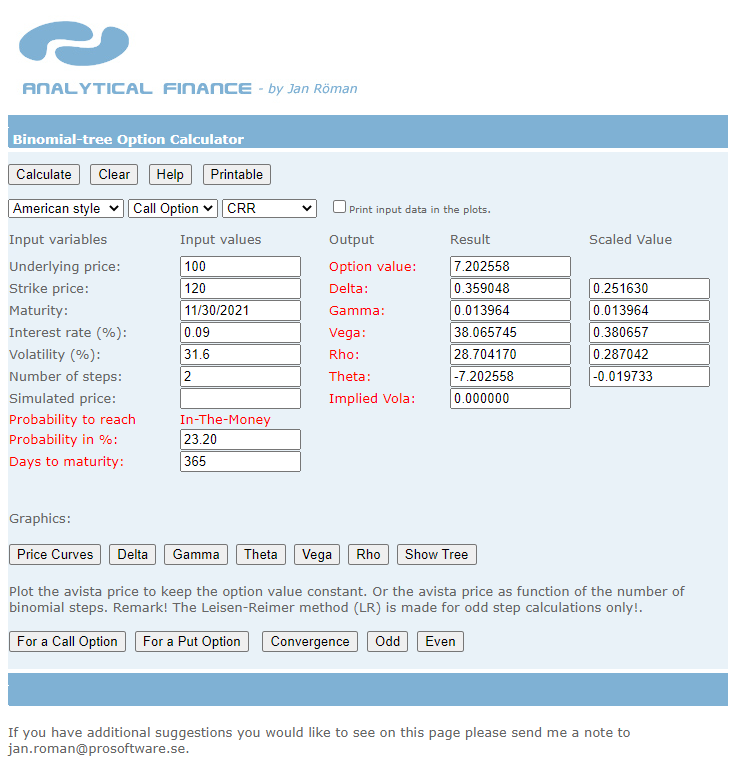
\includegraphics[scale=0.8]{Roman_binomial_calculator_inputs}
  \caption{Roman's Binomial Options Calculator Inputs}
\end{figure}

\begin{figure}[H]
  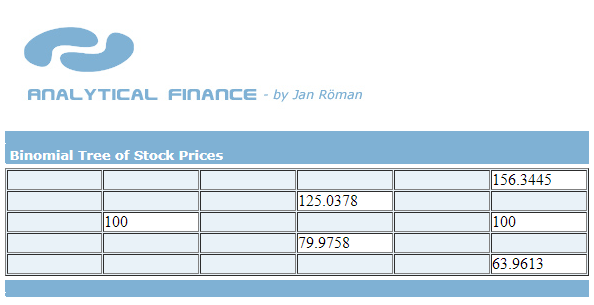
\includegraphics{Roman_binomial_calculator_stock_prices}
  \caption{Roman's Binomial Options Calculator Stock Prices}
\end{figure}

\begin{figure}[H]
  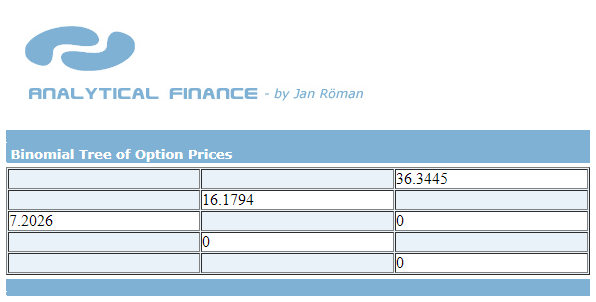
\includegraphics{Roman_binomial_calculator_option_values}
  \caption{Roman's Binomial Options Calculator Option Values}
\end{figure}

When comparing the results of Roman's calculator with the results of our example binomial tree, we can see that both stock and options values generated are very close.
The small differences of precision could be due to the rounded values, but overall, the results are near identical.

\section*{Application}
A binomial options pricing model program written in Python3 was made as the application for this project.
The program created follows and uses the methods and formulas described in this paper and can do a much larger number of steps.

The source code for this application can be found in the same repository that houses the .tex file of this PDF, accessible here:

\href{https://github.com/cliuj/binomial-options-pricing-model}{\color{blue}{https://github.com/cliuj/binomial-options-pricing-model}}

% It's too much of a pain to learn about BibTex, so I'm writing the old-fashion way
\begin{thebibliography}{9}
  \bibitem{derivativefinancewikipedia}
    "Derivative (finance)".
    \\
    \href{https://en.wikipedia.org/wiki/Derivative\_(finance)}{https://en.wikipedia.org/wiki/Derivative\_(finance)}

  \bibitem{blackscholesmodelwikipedia}
    "Black-Scholes Model".
    \\
    \href{https://en.wikipedia.org/wiki/Black-Scholes\_model}{https://en.wikipedia.org/wiki/Black-Scholes\_model}

  \bibitem{bopmwikipedia}
    "Binomial options pricing model".
    \\
    \href{https://en.wikipedia.org/wiki/Binomial\_options\_pricing\_model}{https://en.wikipedia.org/wiki/Binomial\_options\_pricing\_model}

  \bibitem{volatilityfinancewikipedia}
    "Volatility (finance)".
    \\
    \href{https://en.wikipedia.org/wiki/Volatility\_(finance)}{https://en.wikipedia.org/wiki/Volatility\_(finance)}

  \bibitem{madwikipedia}
    "Average absolute deviation"
    \\
    \href{https://en.wikipedia.org/wiki/Average\_absolute\_deviation}{https://en.wikipedia.org/wiki/Average\_absolute\_deviation}

  \bibitem{continouscompoundingformulawikipedia}
    "Compound interest". \\
    \href{https://en.wikipedia.org/wiki/Compound\_interest}{https://en.wikipedia.org/wiki/Compound\_interest}

  \bibitem{exponentcharacterizationswikipedia}
    "Characterizations of the exponential function". \\
    \href{https://en.wikipedia.org/wiki/Characterizations\_of\_the\_exponential\_function}{https://en.wikipedia.org/wiki/Characterizations\_of\_the\_exponential\_function}
  
  \bibitem{damodaran}
    Aswath Damodaran.
    \textit{Investment Valuation: Tools and Techniques for Determining the Value of Any Asset, Third Edition}.
    [Chapter 5: Option Pricing Theory and Models], 87-110,
    ISBN: \textit{9781118011522},
    (2012)

  \bibitem{thebinomialmodelcornell}
    "The Binomial Model".
    \href{https://pi.math.cornell.edu/~mec/Summer2008/spulido/Binomial.html}{https://pi.math.cornell.edu/~mec/Summer2008/spulido/Binomial.html}

  \bibitem{obaidullahxplaind}
    Obaidullah Jan.
    "Stock Valuation".
    \\
    \href{https://xplaind.com/746919/stock-valuation}{https://xplaind.com/746919/stock-valuation}

  \bibitem{brigidavideo}
    Matt Brigida.
    "FIN 376: Binomial Option Pricing and Delta Hedging".
    3:40-4:25.
    \\
    \href{https://www.youtube.com/watch?v=PZrmOh2nZus}{https://www.youtube.com/watch?v=PZrmOh2nZus}

  \bibitem{crrpaper}
    John Carrington Cox, Stephen Ross, and Mark Edward Rubenstein
    "Option pricing: A simplified approach".
    (1979)

  \bibitem{tbondyield}
    "Daily Treasury Yield Curve Rates".
    \href{https://www.treasury.gov/resource-center/data-chart-center/interest-rates/Pages/TextView.aspx?data=yield}{https://www.treasury.gov/resource-center/data-chart-center/interest-rates/Pages/TextView.aspx?data=yield}


\end{thebibliography}

\end{document}
